\documentclass[conference]{IEEEtran}
\IEEEoverridecommandlockouts
% The preceding line is only needed to identify funding in the first footnote. If that is unneeded, please comment it out.
\usepackage{cite}
\usepackage{amsmath,amssymb,amsfonts}
\usepackage{algorithmic}
\usepackage{graphicx}
\usepackage{textcomp}
\usepackage{xcolor}
\usepackage{hyperref}
\usepackage[utf8]{inputenc}
\usepackage{listings}
\usepackage{float}
\lstset{
	basicstyle=\ttfamily,
	columns=fullflexible,
	frame=single,
	breaklines=true,
	postbreak=\mbox{\textcolor{red}{$\hookrightarrow$}\space},
}

\def\BibTeX{{\rm B\kern-.05em{\sc i\kern-.025em b}\kern-.08em
    T\kern-.1667em\lower.7ex\hbox{E}\kern-.125emX}}

\begin{document}

\title{Projeto PCS5029 - Amazon pet product reviews classification}

\author{\IEEEauthorblockN{1\textsuperscript{st} Eduardo de Andrade Nogueira}
\IEEEauthorblockA{\textit{Escola Politécnica da Universidade de São Paulo (Poli/USP)} \\
São Paulo - SP, Brasil \\
eduardonogueira@usp.br}
}

\maketitle

\begin{abstract}
Este resumo apresenta a metodologia utilizada na resolução do problema de classificação de texto de avaliação de produtos de PETs. A base de dados e as descrições do desafio Kaggle onde foi proposto este problema pode ser visto no \href{https://www.kaggle.com/c/amazon-pet-product-reviews-classification/overview}{LINK}
\end{abstract}

\begin{IEEEkeywords}
NLP, WordTokenizer, MultiLayer Perceptron, Support Vector machine, K-Nearest Neighbors, Decision Tree
\end{IEEEkeywords}

\section{Introdução}

Este trabalho tem como objetivo a resolução do desafio do Kaggle de identificar por meio do review dos clientes de um produto de pet obtido do site da Amazon, para qual categoria de animal ele está destinado. Abaixo observa-se alguns exemplos de reviews para cada uma das classes presente no Dataset:

\begin{itemize}
	\item \textbf{Birds} - My little Cockatiel Remus (Remy) loves it! He adores the flower, which I called Alien because it looks like a UFO sorta...just found out it was supposed to be a flower. Its his favorite one!
	
	\item \textbf{Bunny Rabbit Central} - Our piggy had a plastic bowl and she would always knock it over. This one is much deeper, holds more feed \& she doesnt knock it over like she did the plastic.
	
	\item \textbf{Cats} - My cats do not like this toy. I've had it for a few weeks and never see them playing with it. I would not recommend it.
	
	\item \textbf{Dogs} - Sam has an everlast treat each nite before bed, like a good tooth brushing. The only downside is finding a place that keeps them in stock as well as multiple flavors.
	
	\item \textbf{Fish Aquatic Pets} - This is my second one and I love it. Keeps the tank clean.The main problem is once you take the cover off to replace the filter I could never get it to fit right again. but still a good buy.
	
	\item \textbf{Small Animals} - Our rescue rat, George, really likes this food. (He prefers this to lab pellets. And seeded diets are not recommended.) Good quality and healthy. Well worth the money. Oxbow is a good brand.
	
\end{itemize}

Nas próximas seções é apresentado a metodologia usada para a solução do problema, bem como os resultados obtidos com a metodologia proposta.

\section{Resolução do problema}

	\subsection{Limpeza dos dados}\label{sec:CleanData}
	
		\begin{itemize}
			\item \textbf{LowerCase:} Um exemplo da aplicação da transformação LowerCase pode ser observado abaixo:
			\begin{itemize}
				\item \textbf{String Original:}  ESTOU TODO MAIUSCULO
				\item \textbf{String Modificada:}  estou todo maiusculo
			\end{itemize}

			\vspace{0.2cm}
			\item \textbf{Remoção de espaços:} Um exemplo da remoção de espaços na string pode ser observado abaixo:

			\begin{itemize}
				\item \textbf{String Original:} EU    TENHO     MUITO     ESPAÇO
				\item \textbf{String Modificada:} EU TENHO MUITO ESPAÇO
			\end{itemize}
			
			\vspace{0.2cm}
			\item \textbf{Remoção de número junto com texto:} Um exemplo da remoção de número junto ao texto na string pode ser observado abaixo:

			\begin{itemize}
				\item \textbf{String Original:} EssaStringTemNUMEROS289
				\item \textbf{String Modificada:} EssaStringTemNUMEROS
			\end{itemize}
		
			\vspace{0.2cm}
			\item \textbf{Remoção de pontuação: } Um exemplo da remoção de pontuação na string pode ser observado abaixo:
			
			\begin{itemize}
				\item \textbf{String Original:} EU.TENHO.MUITA.PONTUAÇÃO
				\item \textbf{String Modificada:} EU TENHO MUITA PONTUAÇÃO
			\end{itemize}
			
			\vspace{0.2cm}
			\item \textbf{Remoção de StopWords:} Um exemplo da remoção de StopWords na string pode ser observado abaixo:
			
			\begin{itemize}
				\item \textbf{String Original:} all i want to do is remove this stopwords
				\item \textbf{String Modificada:} want remove stopwords
			\end{itemize}
			
			\vspace{0.2cm}
			\item \textbf{Remoção de Underline "\_":} Um exemplo da remoção de underline na string pode ser observado abaixo::

			\begin{itemize}
				\item \textbf{String Original:} ESTOU\_REMOVENDO\_ESSES\_UNDERLINES
				\item \textbf{String Modificada:} ESTOU REMOVENDO ESSES UNDERLINES
			\end{itemize}		
			
			\vspace{0.2cm}
			\item \textbf{Remoção de URLs:} Um exemplo da remoção de URL na string pode ser observado abaixo:
			\begin{itemize}
				\item \textbf{String Original:} Vou remover urls http://www.vouserremovido.com
				\item \textbf{String Modificada:} Vou remover urls
			\end{itemize}
		
		\end{itemize}
	
	\subsection{Word Tokenizer}
		Com o objetivo de converter as strings de atributos em vetores onde é possível aplica-los nos classificadores foi utilizado a biblioteca CountVectorizer do SKLearn que transforma as strings em matrizes matrizes. 
	
	\subsection{Pipeline de teste e métricas de avaliação}\label{sec:pipeline}
		O CountVectorizer, possibilita a seleção da quantidade de elementos no vetor, neste trabalho foi testado doze situações diferentes: 16, 32, 64, 128, 256, 512, 1024, 2048, 4096, 8192, 16384, 32768 e aplicado os classificadores, Perceptron Multicamadas (MLP), Máquina de vetor de suporte (SVM), K-Próximos Vizinhos (KNN) e Árvore de Decisão (DT).
		
		
		As métricas de avaliação usadas neste trabalho foram: Acurácia, Recall, Precisão e F1.
		
%		os quais são dados respectivamente pelas equações \ref{eq:ACC}, \ref{eq:REC}, \ref{eq:PR} e \ref{eq:F1}:
%		
%		\begin{equation}\label{eq:ACC}
%			ACC = \frac{TP + TN}{TP + FP + TN + FN}
%		\end{equation}
%		
%		\begin{equation}\label{eq:REC}
%			RE = \frac{TP}{TP + FN}
%		\end{equation}
%		
%		
%		\begin{equation}\label{eq:PR}
%			PR = \frac{TP}{TP + FP}
%		\end{equation}
%		
%		
%		\begin{equation}\label{eq:F1}
%			F1 = \frac{2.PR.RE}{PR + RE}
%		\end{equation}
	
	\subsection{Avaliação da performance dos classificadores}
	
	
	Após realizado o teste proposto na seção \ref{sec:pipeline} de variação do tamanho do vetor de saída do CountVectorizer, os resultados foram dispostos de forma gráfica nessa seção, onde é possível observar as quatro métricas usadas (Acurácia e o Score F1), respectivamente nas imagens \ref{fig:acc} e \ref{fig:f1}.
	
	\begin{figure}[H]
		\centering
		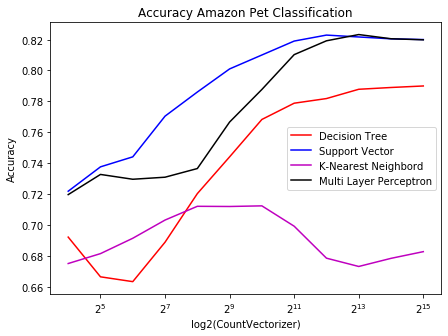
\includegraphics[width=\linewidth]{Images/ACC}
		\caption{Acurácia no teste de classificação de produtos de PET}
		\label{fig:acc}
	\end{figure}

%	\begin{figure}[!htb]
%		\centering
%		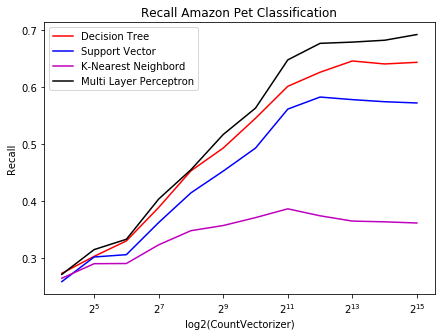
\includegraphics[width=\linewidth]{Images/RE}
%		\caption{Recall no teste de classificação de produtos de PET}
%		\label{fig:re}
%	\end{figure}
%	
%	\begin{figure}[!htb]
%		\centering
%		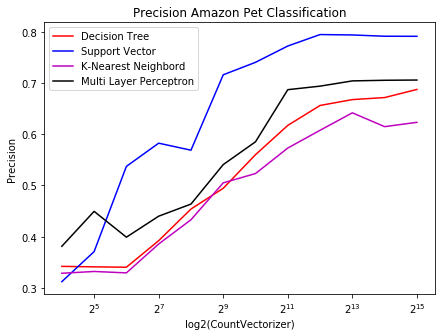
\includegraphics[width=\linewidth]{Images/PR}
%		\caption{Precisão no teste de classificação de produtos de PET}
%		\label{fig:pr}
%	\end{figure}

	\begin{figure}[H]
		\centering
		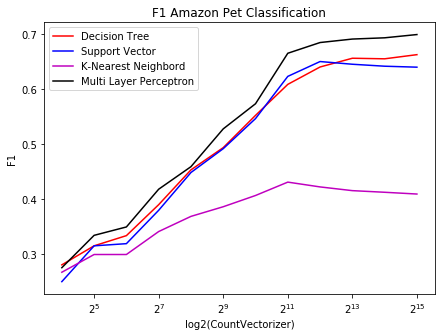
\includegraphics[width=\linewidth]{Images/F1}
		\caption{F1 no teste de classificação de produtos de PET}
		\label{fig:f1}
	\end{figure}


Analisando a acurácia obtida em conjunto com o Score F1, pode-se afirmar que a melhor configuração de classificador é o Perceptron Multi Camadas (MLP) com o CountVectorizer com 8192 features.

\section{Resultado desafio Kaggle}

Após aplicado a metodologia descrita neste resumo, o resultado foi submetido ao Kaggle para avaliação obtendo um score de 0.80947 o qual é obtido pela micro-averaged da pontuação F1.


\begin{figure}[!htb]
	\centering
	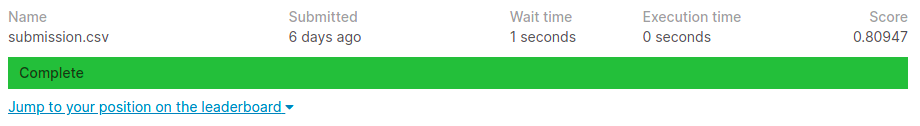
\includegraphics[width=\linewidth]{Images/ResultadoKaggle}
	\caption{Resultado Kaggle}
	\label{fig:resultadokaggle}
\end{figure}


\section{Conclusão}

Após a limpeza dos dados apresentado na seção \ref{sec:CleanData}, foi aplicado o pipeline de testes a fim de se obter a melhor configuração de classificador e tamanho do CountVectorizer. A seleção da melhor configuração foi realizada por meio da acurácia obtida e do score F1.

Após selecionado o melhor classificador como o Perceptron Multi Camadas e o tamanho do vetor do CountVectorizer como tendo 8192 features, o resultado foi submetido ao Kaggle obtendo um score de 0,80947 atingindo o objetivo deste trabalho de classificar para qual pet estava destinado o review.

	
\section{Acesso ao código e a base de dados}

Os links para acessar o código e a base de dados usadas no desenvolvimento deste trabalho estão abaixo:

\begin{itemize}
	\item \textbf{Código Fonte - } https://github.com/eduardoanog/Projeto-PCS5029
	\item \textbf{Base de dados - } https://www.kaggle.com/c/amazon-pet-product-reviews-classification/overview
\end{itemize}


\begin{thebibliography}{00}
\bibitem{b1} Glorot, Xavier, and Yoshua Bengio. "Understanding the difficulty of training deep feedforward neural networks." Proceedings of the thirteenth international conference on artificial intelligence and statistics. 2010.

\bibitem{b2} Chang, Chih-Chung, and Chih-Jen Lin. "LIBSVM: A library for support vector machines." ACM transactions on intelligent systems and technology (TIST) 2.3 (2011): 1-27.

\bibitem{b3} Zhang, Zhongheng. "Introduction to machine learning: k-nearest neighbors." Annals of translational medicine 4.11 (2016).

\bibitem{b4} Breiman, Leo. "Random forests." Machine learning 45.1 (2001): 5-32.
\end{thebibliography}
\end{document}
